\documentclass[addpoints]{exam}
\usepackage[utf8]{inputenc}
\usepackage[russian]{babel}
\usepackage[OT1]{fontenc}
\usepackage{amsmath}
\usepackage{amsfonts}
\usepackage{amssymb}
\usepackage{graphicx}
\usepackage{listings}
\usepackage{algorithm}
\usepackage{algpseudocode}
\usepackage{tikz}
\usetikzlibrary{matrix}
\usepackage{geometry}
 \geometry{
 a4paper,
 total={210mm,297mm},
 left=20mm,
 right=20mm,
 top=20mm,
 bottom=20mm,
 }

\newcommand{\var}[1]{{\ttfamily#1}}
\title{Кратчайшие пути. Остовы. Потоки.}
\author{Минский ШАД. Весна}

../../tasks/common/preamble.tex

\DeclareMathOperator{\Flow}{Flow}
\DeclareMathOperator{\CostFlow}{CostFlow}

\newcommand{\kitten}{%
  \raisebox{-0.7\totalheight}{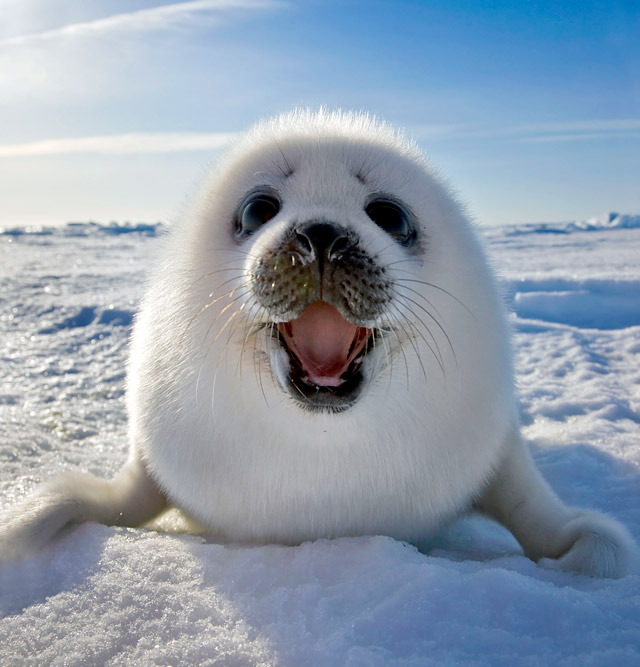
\includegraphics[scale=0.04]{kitten.jpg}}%
}
\newcommand{\cross}{%
  \raisebox{-0.7\totalheight}{
\includegraphics[scale=0.7]{cross.png}}%
}
\newcommand{\mycircle}{%
  \raisebox{-0.7\totalheight}{
\includegraphics[scale=0.2]{circle.jpeg}}%
}

\begin{document}

%\printanswers
\maketitle

\section{Примечание}

В некоторых задачах вам потребуется использовать алгоритмы поиска максимального потока. Если ваш граф не является двудольным в общем случае, то можно просто говорить, что алгоритм имеет сложность $\O{\Flow(n,m)}$, если вам нужно один раз найти максимальный поток в $(n,m)$-графе. В случае максимального потока минимальной стоимости используйте обозначение $\O{\CostFlow(n,m)}$. В случае двудольных графов требуется приводить точную оценку.

\section{Тематические задачи}

\begin{questions}

\question[2 \half] Дан ориентированный $(n,m)$-граф. На каждой дуге написан неотрицательный вес. Необходимо найти все дуги, которые обязательно лежат на кратчайшем пути из $A$ в $B$ (т.е. любой кратчайший путь из $A$ в $B$ их содержит). Время работы алгоритма должно составлять $\O{m \log{n}}$.
  
\begin{solution}

Найдём все дуги, которые вообще могут лежать на кратчайшем пути из $A$ в $B$. Для этого пустим алгоритм Дейкстры из вершины $A$ (пусть он нашёл вектор расстояний $d_A$) и алгоритм Дейкстры из вершины $B$ по транспорированному графу (его вектор~--- $d_B$). Тогда ребро $e=(u,v)$ может лежать на кратчайшем пути если и только если $d_A[u] + cost_e + d_B[v] = d_A[B]$. Оставим только такие дуги графа. На самом деле этот шаг необязателен, просто так легче понимать решение.

Найдём любой кратчийший путь из $A$ в $B$, дуги этого пути назовём красными. Очевидно, что все искомые дуги~--- красные, обратное не всегда верно. Давайте будем проверять каждую из этих дуг на необходимость. Пронумеруем вершины найденного пути по порядку, т.е. вершине $A$ дадим номер $1$, следующей за ней вершине~--- номер $2$, и так далее. Вершине $B$ дадим номер $k$, где $k$~--- количество вершин в найденном кратчайшем пути. Вершинам, которые не лежат на кратчайшем пути выдадим номер ноль.

Затем можно ввести функцию $f[x]$~--- максимальный номер вершины, в которую можно попасть, если идти только по дугам, которые не являются красными (напомню, что мы удалили все дуги, которые не могут лежать на кратчайшем пути из $A$ в $B$). Как её считать? Очевидно, что $f[x]$ это либо номер самой вершины $x$, либо максимум из $f[y]$, где $y$~--- вершина, что есть не красная дуга из $x$ в $y$. Для вычисления можно использовать либо рекурсию с мемоизацией, либо отсортировать изначально вершины по $d_A[x]$.

Пусть мы хотим проверить красную дугу $e=(u,v)$ на необходимость. Предположим, что она не является необходимой. Рассмотрим кратчайший путь, который её не содержит. Он до какого-то момента идёт по пронумерованным вершинам, затем уходит с них, затем возвращается обратно (возможно, несколько раз). Наша задача проверить, можно ли как-то уйти с красного пути до вершины $u$, а затем вернуться после вершины $v$. Очевидно, что для этого необходимо и достаточно, чтоб существовала вершина красного пути с номером не больше, чем $u$, для которой $f$ не меньше, чем номер вершины $v$. Это легко посчитать, накопив префиксный максимум величины $f$ по красному пути.

\end{solution}  
  
\question[2] Дан неориентированный $(n,m)$-граф. Необходимо для каждого ребра найти вес минимального остовного дерева, которое содержит это ребро. Весь алгоритм должен иметь сложность $\O{m \log{m}}$.

Например, на следующих рисунках показаны искомые деревья одного и того же графа для рёбер $(3,4)$ и $(1,3)$ соответственно:

\begin{figure}[h!]
\centering
\begin{minipage}{.5\textwidth}
  \centering
\begin{center}
\begin{tikzpicture}[-,>=stealth',shorten >=1pt,auto,node distance=3cm,
  thick,main node/.style={circle,fill=green!20,draw,font=\sffamily\Large\bfseries}]

  \node[main node] (1) {1};
  \node[main node] (2) [below left of=1] {2};
  \node[main node] (3) [below right of=2] {3};
  \node[main node] (4) [below right of=1] {4};
  \node[main node] (5) [right of=1] {5};

  \path[every node/.style={font=\sffamily\small}]
    (1) edge node [above] {10} (5)   
        edge node [right] {6} (3)   
    (2) edge [red,line width=1.3]  node [left,black] {15} (1)
    (3) edge [right,red,line width=1.3] node[left,black] {10} (4)
    (4) edge [right,red,line width=1.3] node[right,black] {5} (1)
        edge [right,red,line width=1.3] node[right,black] {8} (5)
    ;
\end{tikzpicture} 
\end{center}
\end{minipage}%
\begin{minipage}{.5\textwidth}
  \centering
\begin{center}
\begin{tikzpicture}[-,>=stealth',shorten >=1pt,auto,node distance=3cm,
  thick,main node/.style={circle,fill=green!20,draw,font=\sffamily\Large\bfseries}]

  \node[main node] (1) {1};
  \node[main node] (2) [below left of=1] {2};
  \node[main node] (3) [below right of=2] {3};
  \node[main node] (4) [below right of=1] {4};
  \node[main node] (5) [right of=1] {5};

  \path[every node/.style={font=\sffamily\small}]
    (1) edge node [above] {10} (5)   
        edge [red,line width=2] node [right,black] {6} (3)   
    (2) edge [red,line width=1.3] node [left,black] {15} (1)
    (3) edge [left] node[left,black] {10} (4)
    (4) edge [right,red,line width=1.3] node[right,black] {5} (1)
        edge [right,red,line width=1.3] node[right,black] {8} (5)
    ;
\end{tikzpicture} 
\end{center}
\end{minipage}
\end{figure}

\question[2 \half] Дан взвешенный $(n,m)$-граф. Весом пути будем называть вес самого тяжёлого ребра пути. Найти вес кратчайшего пути из вершины $A$ в вершину $B$ за $\O{m}$. 

\question[1] \label{dijk} Дан взвешенный $(n,m)$-граф без отрицательных рёбер. Вам разрешается заменить вес $k$ любых рёбер на произвольное неотрицательное число (вес разных рёбер можно менять на вес разные числа) Вам нужно найти кратчайший (по сумме весов рёбер) путь из вершины $A$ до вершины $B$ за время $\O{m + n\log{n}}$. Число $k$ считать константой. 

\question[2] Дан взвешенный $(n,m)$-граф без отрицательных рёбер. Чтоб пройти ребро с весом $w$ необходимо ровно $w$ минут. На этом графе расположено $k$ студентов, $i$-й студент изначально находится в вершине $s_i$. Все студенты хотят добраться до вершины с номером $1$, потому что там расположена общага, которая вот уже скоро закроется. Студенты понимают, что если они пойдут не по кратчайшему пути, то до закрытия уже не успеют. Поэтому, если некоторый студент понимает, что он не сможет пройти по кратчайшему пути, то он просто разочаровывается в жизни, уходит из графа, садится на асфальт и начинает плакать. Кроме того, если два студента в какой-то момент времени окажутся в одной точке одного и того же ребра, то они начнут спорить про условия теоремы Куна-Такера и оба опаздают в общагу. Замечу, что по народной примете, спорить можно только на рёбрах, поэтому если два студента встречаются в вершине, но потом уходят по разным рёбрам, то спора не происходит. Студенты ходят по рёбрам с одинаковой скоростью и проводят на вершинах нулевое время. Какое максимальное количество студентов могут попасть сегодня в общагу? Ваш алгоритм должен иметь сложность $\O{n \log{n} + km}$

К примеру рассмотрим следующий граф:

\begin{center}
\begin{tikzpicture}[-,>=stealth',shorten >=1pt,auto,node distance=3cm,
  thick,main node/.style={circle,fill=yellow!20,draw,font=\sffamily\Large\bfseries}]

  \node[main node] (1) {1};
  \node[main node] (2) [below of=1] {2};
  \node[main node] (3) [below right of=1] {3};
  \node[main node] (4) [right of=1] {4};

  \path[every node/.style={font=\sffamily\small}]
    (1) edge node [left] {5} (2)
        edge node [below] {4} (3)
    (3) edge node [right] {6} (4)
    (4) edge [bend left=80] node [below] {5} (2)
        edge node [below] {11} (1)
    ;
\end{tikzpicture}
\end{center} 

И пусть $4$ студента стоят в вершине $4$, один студент~--- в вершине $1$, а в остальных вершинах вообще нет студентов. Тогда ответ на задачу $3$. Действительно, студент, который и так в общаге, никому не помешает. А вот из четырёх студентов из $4$-й вершины добраться, не помешав друг другу могут только два. Один пойдёт по пути $4-3-1$, другой по $4-2-1$. По ребру $(1,4)$ никакой студент пойти не захочет, так как это не кратчайший путь.

\question[2] \label{scc} У малыша Чингиса, как известно, было много сыновей. Но задача только про $N$ из них. Известно, что в один прекрасный день он повелел собрать ровно $N$ самых красивых девушек со всех своих земель и привести их к себе. После этого он сказал своему главному мудрецу: <<зафигачь так, чтоб у каждого сына было ровно по одной девушке, но так, чтоб все сыновья были довольны, в частности, каждая девушка должна быть ровно у одного сына>>. Для начала мудрец спросил у каждого сына, какие из девушек ему понравились. $i$-й сын сказал: <<ну, короче, вот эти $k_i$ ничего так, т.е. с номерами $a_{i,1}, a_{i,2}, \ldots, a_{i,k_i}$. С другими~--- хоть убей, не буду>>. Мудрец, не мудрствуя лукаво, почитал свою любимую скрижаль за авторством малыша Тома и понял, что нужно в некотором несложном графе найти совершенное паросочетание. Он подумал ещё немного, попробовал~--- и у него получилось. Вернувшись к малышу Чингису, он сказал: <<смотри, тема такая: $i$-й сын берёт $w_i$-ю девку, и порешили>>. Но Чингис оказался не так прост. Он сказал: <<может нет? Может давай лучше сын с номером $x$ возьмёт себе девушку с номером $y$? Иди думай над таким вариантом>>. Мудрец понял, что так легко он не отделается. Поэтому он решил по числу $N$, векторам $a_i$ и вектору $w$ найти для каждого $x$, каких девушек он может забрать, чтоб остальные $N-1$ девушек можно было распределить между остальными $N-1$ сыном. Сделать это надо за $\O{\max(T, N + A)}$, где $T$~--- размер ответа, а $A = \sum\limits_{i=1}^N k_i$. 

\question[2] \label{max_flow} Малыш Тик и малыш Так играют в игру крестики-нолики на поле $N \times M$. Игра происходит следующим образом. Сначала, для интереса, в некоторые клетки садят очень спокойных котят. Котята никогда не уходят с этой клетки, поэтому ходить в эти клетки нельзя. Игроки ходят по очереди, начиная с крестиков. Игра заканчивается, когда на поле не остаётся пустых клеток, либо когда на поле появляется строка без пустых клеток или столбец без пустых клеток, в которых ноликов строго больше, чем крестиков, либо крестиков строго больше, чем ноликов. Если после окончания игры есть заполненный столбец или строка, в которой одной фигуры больше, чем другой, то игрок, играющий этой фигурой объявляется победителем. Иначе игра оканчивается ничейным результатом. Малыш Тик гораздо старше малыша Так и всегда выигрывал у него. Лишь вчера малышу Таку удалось свести одну партию вничью. И всё бы ничего, но чтоб произвести впечатление на малышку Тоу, ему хочется показать поле той легендарной партии. Но вот незадача, некоторые из котиков чихнули и стёрли часть фигур. Тем не менее, они настолько спокойны, что остались на своих местах. Теперь задача Така состоит в том, чтоб расставить фигуры на стёртые места таким образом, чтоб образовывалось поле, которое могло получиться в результате ничейной игры.

Например, если поле вот такое:

\begin{center}
\begin{tabular}{|c|c|c|}
\hline 
\cross &  & \kitten \\ 
\hline 
 & \kitten &  \\ 
\hline 
\kitten &  &  \\ 
\hline 
\kitten & \kitten & \kitten \\ 
\hline 
\end{tabular} 
\end{center}

То из него могло получиться следующее:

\begin{center}
\begin{tabular}{|c|c|c|}
\hline 
\cross & \mycircle  & \kitten \\ 
\hline 
\mycircle & \kitten & \cross  \\ 
\hline 
\kitten & \cross  & \mycircle  \\ 
\hline 
\kitten & \kitten & \kitten \\ 
\hline 
\end{tabular} 
\end{center}

\section{Задачи на повторение}

\question[1 \half]  Дано дерево на $n$ вершинах. Посчитать суммарную длину (по рёбрам) всех простых путей в этом дереве за $\mathcal{O}(n)$.

\question[2] Задано конечное множество $A$. На нём задана функция $f: A \to A$ своей таблицей значений. Найти минимальное натуральное $k$ такое, что $f^k$ идемпотентна или сказать, что такого $k$ не существует. Алгоритм должен иметь сложность $\O{|A| \log{|A|}}$, можно считать, что $A$~--- множество натуральных чисел от $1$ до $|A|$.

\section{Практические задачи}

Ссылка на контест: \url{https://contest.yandex.ru/contest/1080/problems/}

\question[2] Реализуйте решение задачи \ref{dijk}

\question[2] Реализуйте решение задачи \ref{scc}

\question[2] Реализуйте решение задачи \ref{max_flow}

\begin{center}
\pointtable[h][questions]
\end{center}

\end{questions}

\end{document}
